\section{The Resistor Color Code}
\label{resistor_code}

The table below shows how to use the colored bands on a resistor to determine its resistance.  In all cases, the digits come first, then one multiplier band, then one ``tolerance'' band. 


{\centering 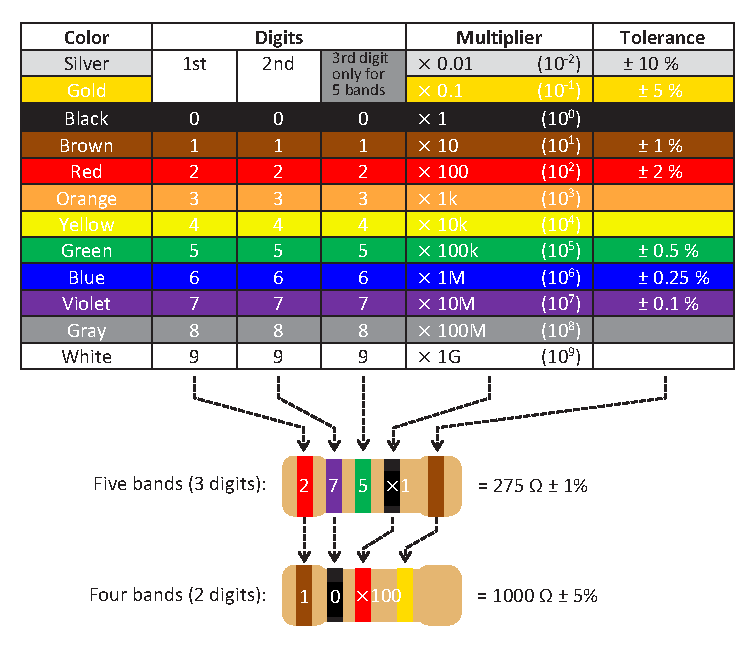
\includegraphics{appendices/resistor_code/resistor_table.eps} \par}
\index{color page}

%Note, not for printing: I have left off the tolerances for Orange (0.05% or 3%), Yellow (0.02% or 4%) and Gray (0.05% or 0.01%).  These values have actually changed over time, but are thankfully rare.  For an apparently gray band, it is much more likely that the band is really intended to be silver (10%).  In fact, in some silver and gold bands, the metallic particles are sometimes left out of the paint to prevent arcing in high-voltage applications, making the paint actually gray or yellow.

The tolerance band tells you something like the ``uncertainty'' of the resistance, but the values are chosen very conservatively because the manufacturer \textit{guarantees} that the value will be within the stated tolerance.  For example, the four-band resistor pictured above is \textit{guaranteed} to be between $950~\Omega$ and $1050~\Omega$.  In practice, you will \textit{never} find a ``5\%'' resistor that is actually off by that much.


\medskip
\textbf{Which Direction to Read? Several Possible Clues:}
\begin{itemize}[nosep]
\item Sometimes the first digit is closer to the one of the resistor than the tolerance band is.  If so, start there.
\item Sometimes there is extra space between the multiplier and tolerance bands, as in the drawings above.  If you see that extra space, start on the other side.
\item Gold and Silver are never digits; they are always tolerance or multiplier bands.  If you see gold or silver, start on the other side.
\end{itemize}

\medskip
\textbf{Variations and a Caution}

There are rare variations to the code above.  Occasionally an additional band will denote the temperature coefficient or a failure rate.  There are also rare cases of orange, yellow, or gray tolerance bands, which can have multiple interpretations.  Finally, be warned: on very small bands, it is easy to confuse orange/red, red/brown, or violet/gray.  (Fortunately, you can usually measure a resistor with your multimeter and know for sure!)

\medskip
\textbf{Mnemonic Devices}

There are several fun phrases (and some not-so-fun ones) you can memorize to help you remember the order of the colors.   In the ones below, the vowels also help distinguish between Black/Brown/Blue and Green/Gray.
\begin{itemize}[nosep]
%\item \textbf{Ba}d \textbf{Bo}sses \textbf{R}ely \textbf{O}n \textbf{Y}oung \textbf{Gee}ks, \textbf{Bu}t \textbf{V}alue \textbf{Grea}t \textbf{W}ork.
\item \textbf{Ba}d \textbf{Bo}ss \textbf{R}elies \textbf{O}n \textbf{Y}our \textbf{Ge}nius, \textbf{Bu}t \textbf{V}iews \textbf{Grea}tness \textbf{W}arily.
\item \textbf{Bla}nd \textbf{Bo}oks \textbf{R}eportedly \textbf{O}ptimize \textbf{Y}our \textbf{GRE}, \textbf{Bu}t \textbf{V}ideo \textbf{Ga}mes \textbf{W}on't.
\end{itemize}

